% !TEX root = ../main.tex
\section{Benchmarks}\label{sec:benchmarks}

%\gnote{Tables may need to change to accommodate updated aggregate signature size. Possibly also need to update non-aggregate sizes and sigs because optimization gives different params}

In this section, we define the parameters with which we instantiate Chipmunk and we provide various benchmarks, showing that our new construction significantly outperforms the previous Squirrel construction of Fleischhacker, Simkin, and Zhang~\cite{CCS:FleSimZha22}.

Our concretely proposed construction uses the key-homomorphic one-time signature scheme for \autoref{fig:otsconstruction} and \eprint{$\hvcencoded$}\cameraready{$\hvccamera$} for the homomorphic vector commitment.

\subsection{Parameters and Security Estimates}
The dimension of the ring $\ring$ is fixed to $n=512$. We choose $q,q'$, s.t.\ $q,q'\equiv 1\mod 2n$, in order speed up multiplications in $\ring_q$ and $\ring_{q'}$ by using NTT.
The constraints that need to be satisfied by our parameters are summarized in Table \ref{tab:constraints}.
The concrete efficiency for a given set of parameters is determined by Table \ref{tab:efficiencyfromparameters}, which also spells out where the contributions come from.
To find such concrete parameters we used a script\footnote{\label{fn:github}\url{https://github.com/GottfriedHerold/Chipmunk}}, which enumerates possible parameters that satisfy all constraints, that lead to hard ring-SIS problems, and that allow for efficient NTT evaluations.
For any choice of $\secpar\in\{112,128\}$, $\rho\in\NN$, and $\tau\in\NN$ our script finds the parameter set that allows for the smallest possible signature size.
For convenience, the results of running the script for a range of reasonable input parameters are shown in \autoref{tab:param} in Appendix~\ref{sec:concreteparams}.%\gnote{@Zhenfei: The bound from \autoref{lem:hvcprobhom} has changed; may need to re-run.}
\begin{table}
  \centering
  \begin{tabular}{@{\makebox[3em][r]{\rownumber\space}} l@{\hspace{3em}}rl}
  \toprule
   \multicolumn{1}{@{\makebox[3em][r]{\#\space}} c}{Source}&\multicolumn{2}{c}{Constraint}\\
  \midrule
   \autoref{lem:hvcprobhom}&$\bagg \geq$&$ \eta\sqrt{2\alpha_w\rho(\ln \frac{2n}{\errorbound} + \ln(2\tau \kappa + \xi\kappa' \eprint{+ 2\tau}))}$\\
   \autoref{lem:hvcprobhom}&$\kappa=$&$\ceil{\log_{2\eta+1}q}$\\
   \autoref{lem:hvcprobhom}&$\kappa'=$&$\ceil{\log_{2\eta+1}q'}$\\
   \autoref{thm:EncodingOfOpenings}& $\beta_{\texttt{encode}}<$ &$\frac{\bagg}{2\eta} + 1/2$ \\
   \autoref{lem:kots_correct}& $\beta_\sigma \geq$&$ 4\varphi\alpha_H\sqrt{\tfrac{1}{2}\alpha_w\rho \cdot \ln \frac{2n\otspkkeylen}{\errorbound} }$\\
   \autoref{lem:kots_sis}&$\abs{\tern_{\alpha_H}} \geq$&$ 2^{2\secpar}$\\
   \autoref{lem:keyhidden}& $\otspkkeylen\geq$&$((3\secpar+\delta)/n+\log_2q')\log^{-1}_2(\varphi+\tfrac{1}{2})$\\
   \autoref{lem:keyhidden}& $\abs{\tern_{\alpha_H}} \leq$&$ 2^{2\secpar + \delta}$\\
   \autoref{lem:nilssupportivechildsupport}&$q'>$&$ 16 \alpha_w \alpha_H\varphi$\\
   \autoref{def:actual_chipmunk}&$\xi=$& $2$\\
   \autoref{lem:msigaggcorrect}&$\chi \geq$ &$\secpar/\log(\tfrac{1}{2\errorbound})$\\
   \autoref{lem:msigunf}&$\abs{\tern_{\alpha_w}} \geq$&$2^\secpar$\\
  %\bottomrule
  \end{tabular}
%   \gnote{$\xi = 2\otspkkeylen$ is missing, from the connection of the HVC and KOTS. I suggest renaming $\otspkkeylen$, anyway.}
  \caption{The constraints a set of Chipmunk parameters needs to satisfy to ensure that the proofs are applicable. The parameters additionally need to be chosen such that the associated Ring-SIS problems are hard.}\label{tab:constraints}
  \end{table}
  
\begin{table}
 \centering
 \begin{tabular}{ll@{\hskip 4ex}l}
  \toprule
  Contribution & & Size in Bits\\
  \midrule
  \multirow{2}{*}{public parameters} & HVC: Ajtai's hash functions & $n(\xi\limbs' + 2\limbs)\ceil{\log q}$\\\cline{2-3}
                                     & KOTS & $n \otspkkeylen \ceil{\log q'}$\\
  \hline                                  
  public key                         & HVC commitment & $n\ceil{\log q}$\\
  \hline
  secret key                         & $2^\tau$ KOTS keys & (may regenerate on the fly)\footnoteref{fn:onlinekeys}\\
  \hline
  \multirow{2}{*}{signatures (individual)} & KOTS signature & $n \otspkkeylen\ceil{\log(4\varphi\alpha_H + 1)}$\\\cline{2-3}
                                          & HVC opening   & $(\tau\limbs + \xi\limbs')n \ceil{\log(2\eta+1)}$\\
  \hline                                         
  \multirow{3}{*}{aggregate signatures} & agg.\ KOTS signature & $n \otspkkeylen \ceil{\log(2\beta_\sigma + 1)}$\\\cline{2-3}
                                        & agg.\ HVC opening & $(\tau(\cameraready{2}\limbs-1) + (\xi\limbs'-1))n\ceil{\log(2\bagg+1)} \eprint{+ \tau\limbs n\normalceil{\log(\lfloor \tfrac{\bagg}{\eta}\rfloor+ 2)}}$\\\cline{2-3}
                                        & index $j$ of aggregation attempt & $\normalceil{\log \chi}$\\
 \hline
 \end{tabular}
 
 %\bigskip % Remove together with gnote
% \gnote{@Zhenfei: Please verify that this matches your scripts}
 
\caption{Space efficiency of Chipmunk as a function of the tunable parameters. $\limbs \coloneqq \ceil{\log_{2\eta+1}q}$, $\limbs'\coloneqq \ceil{\log_{2\eta+1}q'}$ }
\label{tab:efficiencyfromparameters}
\end{table}

  
Let us briefly explain how our script works.
First, to ensure security of Chipmunk, the specific ring-SIS problems in Lemma \ref{lem:hvcprobhom} and \ref{lem:kots_correct} need to be hard.
We use the same approach to derive the security of the parameters as was used in Squirrel \cite{CCS:FleSimZha22}.
We adopt the so-called \enquote{realistic model} from \cite{USENIX:ADPS16}.
For a BKZ of block size $\beta$, the cost in this model is estimated by
$2^{0.292\beta+16.4+\log(\#\texttt{SVP calls})}$. 
The LWE-estimator \cite{DBLP:journals/jmc/AlbrechtPS15}
shows that for a root Hermite factor of $1.005$ we expect a block size of 286, which yields $112$ bits of security under the above model.
Similarly, a root Hermite factor of $1.004$ yields $128$ bits of security.

The output length of the hash function that is used for hashing messages needs to be large enough to prevent meet-in-the-middle type of attacks and from the security proofs we also need that for given public parameter $\vec{a}$, a fixed hash digest in $\tern_{\alpha_H}$, and a signature $\vec{\sigma}$ for the one time signature scheme,
there exists at least two short corresponding $(\vec{s}_0, \vec{s}_1)$ with overwhelming probability.
%Then, on the output of the hash of the message, we need it to be large enough
%to be security against meet-in-the-middle type of attacks; 
%in the meantime, for the security proof,
%we also need to customize $\tern_{\alpha_H}$, such that, 
%for a given public parameter $\vec{a}$, a fixed hash digest in $\tern_{\alpha_H}$,
%and a signature $\vec{\sigma}$ for the one time signature scheme,
%there exists at least two short $(\vec{s}_0, \vec{s}_1)$ with overwhelming probability.
Lastly, we also require every randomizer to be unguessable, and therefore $\abs{\tern_{\alpha_w}} \geq 2^\secpar$.

\subsection{Implementation}
Chipmunk was implemented in Rust. The source code, as well as the scripts for parameter derivation are released to the open domain\footnoteref{fn:github}.

\subsubsection{Comparison.}\label{ss:comparison}
For evaluating the performance of Chipmunk, there are two natural points of reference, which are
the trivial solution of just storing a list of $\rho$ Falcon signatures naively and using
Squirrel~\cite{CCS:FleSimZha22}, the previous state-of-the-art construction.
The data for Chipmunk and Squirrel are collected over a same benchmark platform, an AMD 5900x with 24 threads and 32 Gigabytes of memory.
The data for Falcon-512 is collected from the official website\footnote{\url{https://falcon-sign.info/}}.
All three candidates are instantiated to yield $112$ bits security.

In Table~\ref{tab:benchmarksizes}, we compare the three solutions for a fixed parameters set, where we only change the number of signatures that are being aggregated.
The comparison with the trivial Falcon solution is quite straightforward as the size of the naive solution's aggregated signatures grows linearly in the number of signers.
For an aggregate signature involving $8192$ signers, Chipmunk outperforms the trivial solution by a factor of $40$ in terms of aggregate signature size.
Obviously, the improvement only gets larger as the number of signers increases,
In comparison to Squirrel, we see that for both $1024$ and $8192$ aggregated signatures, our scheme is better in all metrics.
There are two main obstacles, namely the key generation time and the aggregate signature size, that would prevent Squirrel from being widely deployable.
Our benchmarks show that Chipmunk's key generation time is better by a factor of $7.4$ and that the size of the aggregate signatures is smaller by a factor of $5.6$.%\gnote{Needs update}
\bgroup
\setlength{\tabcolsep}{0.5em}
\renewcommand{\arraystretch}{1.1}
\begin{table}\centering
  \begin{tabular}{clccccc}
    \# signers      &                 & Falcon      & Squirrel  & Chipmunk  & Imp. Falcon & Imp. Squirrel \\\toprule
    \multirow{2}{*}{} 
                    & Key Generation  & 8.6 ms      & 4 min     & 32.3 sec  &     -       & 7.4$\times$ \\%\cline{2-7}
                    & Signing         & 0.17 ms     & 2.1 ms    & 0.4 ms    &     -       & 5.2$\times$ \\%\cline{2-7}
                    &Fresh Sig. Size  & 666 Bytes   & 45 KB     & 32 KB     &     -       & 1.4$\times$ \\\midrule
    \multirow{3}{*}{1024}                
                    &Aggregation      & -           & 1.2 sec   & 0.57 sec  &     -       & 2.1$\times$ \\%\cline{2-7}
                    &Batch Verification    
                                      & 36.7 ms     & 19.5 ms   & 7.7 ms    & 4.8$\times$ & 2.5$\times$ \\%\cline{2-7}
                    
                    &Agg. Sig. size   & 682 KB      & 572 KB    & 118 KB    & 5.7$\times$ & 4.8$\times$ \\\midrule
    \multirow{3}{*}{8192}                
                    &Aggregation      & -           & 9.6 sec   & 4.6 sec   &     -       & 2.1$\times$ \\%\cline{2-7}
                    &Batch Verification    
                                      & 294 ms      & 53  ms    &  45 ms    & 6.5$\times$ & 1.2$\times$ \\%\cline{2-7}
                    &Agg. Sig. size   & 5.5 MB      & 762 KB    & 136 KB    & 40 $\times$ & 5.6$\times$\\ \bottomrule
  \end{tabular}
  \caption{Comparison of Chipmunk, Squirrel, and a trivial solution of just concatenating all individual signer's Falcon-512 signatures. Squirrel and Chipmunk are instantiated with $\secpar = 112$ and $\tau=21$. %\gnote{Needs update}
  }\label{tab:benchmarksizes}
\end{table}

\subsubsection{Cost of encoding.}
We benchmark the cost of encoding mechanism. On a single thread, the encoding algorithm takes $7.3 ns$ to convert a single node into its encoded form; and the decoding algorithm takes $6.6 ns$ for the reverse direction.
While the cost of encoding/decoding algorithm itself is negligible compared to the main body of the aggregation and batch verification algorithms; it does have a significant impact on the verification algorithm.
Without our encoding algorithm, the verifier can verify each layer in the $\hvc$ openings in parallel; while when encoding algorithm is adopted, a serial dependency is introduced: the verifier needs to compute the hint from the previous layer before decoding the current layer.
This introduces a trade-off between verification cost and the aggregated signature size, as captured in Table \ref{tab:encode_trade_off}.
\begin{table}[t]\centering
  \begin{tabular}{c|cc|cccc}
    \multirow{2}{*}{Tree Height}   &  \multicolumn{2}{c|}{With Encoding}      & \multicolumn{2}{c}{Without Encoding}  \\\cline{2-5}
                  &   Signature size  & Verification time & Signature size    & Verification time                     \\\toprule
      $21$        &       118 KB      &        8.6 ms     &    142 KB         &      7.3 ms                           \\
      $24$        &       133 KB      &        8.9 ms     &    160 KB         &      7.5 ms                           \\
      $26$        &       143 KB      &        9.4 ms     &    172 KB         &      7.1 ms                           \\\bottomrule

  \end{tabular}\\
  \caption{Trade-off between signature size and verification cost via encoding algorithm. Instantiated with $\lambda = 112$ and $\rho = 1024$.}
  \label{tab:encode_trade_off}
\end{table}

Note that with encoding, although the verification algorithm becomes serial across different layers of the tree, the main computation (i.e., the ring multiplications) within each layer is still parallelization friendly.
Overall, for the platform that we tested (with 24 threads), we only observe a slight decrease in the verification speed compared to non-encoding method. 
We conclude that it is always beneficial to use our encoding mechanism.


\subsubsection{Scalability in terms of $\tau$.}
To investigate Chipmunk's practicality, we take a closer look at the key generation time and the aggregated signature size.
For this purpose, we conducted a benchmark over a typical server that is equipped with an AMD 7773x with 64 cores and 1 Terabytes of memory.
In Table \ref{tab:bench_results}, we show how the efficiency of Chipmunk behaves, when the tree height $\tau$ grows.
Notice that this platform is different from that of \autoref{ss:comparison} and that it more accurately simulates the computational power of real-world nodes running blockchains.

\begin{table}[t]\centering
  \begin{tabular}{ccccccc}
      Tree Height         & Key Generation            & Online Signing\footnotemark        
      & $\#$ Signers  
                                                                                            &  Aggregation & Verification  & Agg. Sig. Size  \\ \toprule
      \multirow{2}{*}{21} & \multirow{2}{*}{9.1 sec}  & \multirow{2}{*}{0.40 ms}  & 1024    &   468 ms     &  8.6 ms       & 118 KB     \\%\cline{4-7}
                          &                           &                           & 8192    &   3.8 sec    &  42.6 ms      & 136 KB     \\\hline

      \multirow{2}{*}{24} & \multirow{2}{*}{37.4 sec} & \multirow{2}{*}{0.44 ms}  & 1024    &   516 ms     &  8.9 ms       & 133 KB     \\%\cline{4-7}
                          &                           &                           & 8192    &   4.1 sec    &  46 ms        & 153 KB     \\\hline

      \multirow{2}{*}{26} & \multirow{2}{*}{  4 min}  & \multirow{2}{*}{0.44 ms}  & 1024    &   630 ms     &  9.4 ms       & 143 KB     \\%\cline{4-7}
                          &                           &                           & 8192    &   4.6 sec    &  51 ms        & 164 KB     \\\bottomrule

  \end{tabular}\\
  \caption{Benchmark results}
  \label{tab:bench_results}
\end{table}
\egroup
\footnotetext{\label{fn:onlinekeys}Similar to Squirrel~\cite{CCS:FleSimZha22}, Chipmunk is an online-offline signature scheme, since the opening of the vector commitment can be computed ahead of time without knowing the message to be signed.
This means that online signing only consists of computing the one-time signature.
The secret key of Chipmunk is a large tree, which can be re-derived from a pseudorandom seed whenever needed.
This is computationally quite expensive, but a signer can trade storage size against offline signing speed by caching the top layers of the tree.
The reported times for signing correspond to the \emph{online} signing time.
}
% \end{table}
% \subsection{Micro Benchmarks}
In~\autoref{fig:keygen}, we also plotted the key generation times and aggregate signature sizes of Chipmunk for a growing tree height $\tau$.
One can see that both of these benchmarks scale linearly in the number of leaves of the tree as expected.
For the largest parameter set with $\tau = 26$ we can generate a keypair in just 4 minutes, significantly improving over the 2 hour key generation time of Squirrel.
Such a key would be sufficient for 21 years of usage assuming each block takes 10 seconds to finalize as in the case of Ethereum. 
We conclude that the key generation time is no longer a bottleneck for practical deployment.
\begin{figure}[H] 
  \centering
  \begin{subfigure}[b]
  {0.49\textwidth}    \centering
  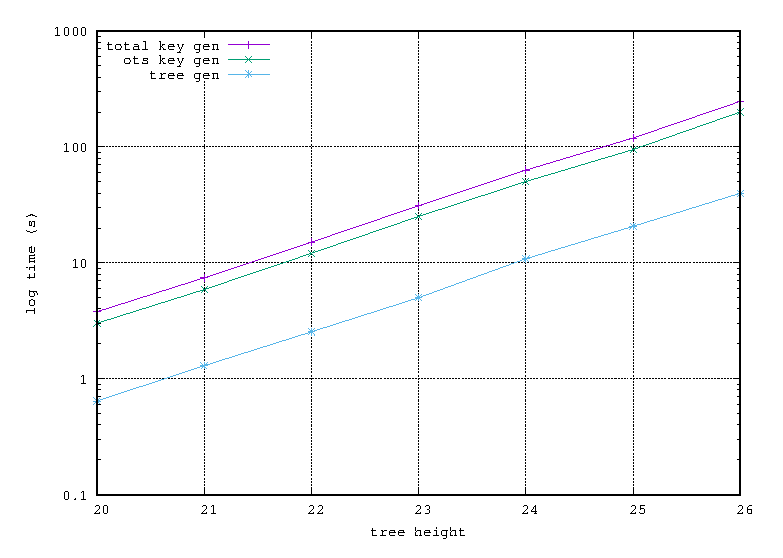
\includegraphics[trim={1mm 0 4mm 0},clip,width=\textwidth]{figures/key_gen.eps}\\
  \caption{Chipmunk key generations time.}
  \end{subfigure}
\begin{subfigure}[b]{0.49\textwidth}    \centering
  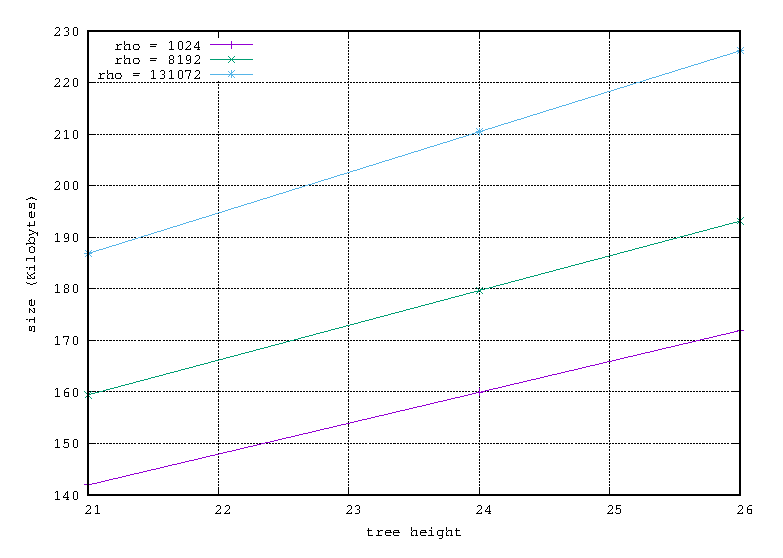
\includegraphics[trim={1mm 0 4mm 0},clip,width=\textwidth]{figures/sig_size.eps}\\
  \caption{Chipmunk aggregated signature size}
  \label{fig:sigize}
  \end{subfigure}
  \caption{Plots showing the scaling characteristics of the key generation time and aggregated signature size of Chipmunk.} \label{fig:keygen}
\end{figure}

\subsubsection{One Aggregate Signature under the Microscope.}

%\mbox{}\gnote{@Zhenfei: Needs rewriting and updating the actual numbers once optimization was run. Please check that it's correct for the camera-ready version}.

To better understand the size of Chipmunk aggregate signatures, we also inspected the sizes of the aggregate signature's individual components.
For the sake of concreteness, let us just consider $\tau=21$ and $\rho=1024$.
An aggregated signature of size approx $118$ Kilobytes,
fitting inside a single ethereum block whose peak size is around 130 Kilobytes\footnote{\url{https://etherscan.io/chart/blocksize}}.
It consists of the following three components.

First, an encoding of the aggregated path and its adjacent nodes. %, as well as the aggregated decomposed public keys.
The aggregated path and its adjacent nodes belong to the homomorphic vector commitment, i.e. $2\tau\limbs$ polynomials in $\ring$ with an infinity norm bound $\bagg$.
We use the encoding method to encode half of those ring elements. Therefore, all these nodes can be represented with $\tau\limbs$ polynomials bounded by $\beta_{\texttt{encode}}$; 
and another $\tau\limbs$ polynomials bounded by $\bagg$. The total size of the path is $\tau\limbs n((\log(\beta_{\texttt{encode}})+1) + (\log(\bagg)+1)) = 102$ Kilobytes.

The aggregated decomposed public keys for the one time signature scheme, i.e., $2\limbs'$ polynomials in $\ring$ with a same norm bound $\bagg$. This requires $2\limbs'n(\log(\bagg)+1)=8$ Kilobytes.

The last component is the aggregated one time signature, i.e., $\otspkkeylen$ polynomials in $\ring$ with norm bound $\beta_\sigma < 2^{20}$, that constitutes $\otspkkeylen n (\log(\beta_\sigma)+1)=8$ Kilobytes. %\gnote{@Zhenfei/Mark:Grammar}

The total size of the aggregated signature is therefore $102 + 8 + 8 = 118$ Kilobytes.
